%ssms

\documentclass[../../main/main.tex]{subfiles}




\begin{document}
\title{Secure State Machine Model}

%%%%%%%%%%%%%%%%%%%%% Chapter SSM Model %%%%%%%%%%%%%%%
\chapter{Secure State Machine Model}\label{chp:ssmmodel}
This chapter introduces the reader to secure state machines (\gls{ssm}s).  It begins with a description of state machines and then describes \textit{secure} state machines.  It concludes with a description of the \gls{hol} implementation of the \gls{ssm}.  After reading this chapter, the reader should be prepared to follow the description of the patrol base operations implementation in \gls{hol} (described in the next chapter).

      %%%%%%%%%%%%%%%%%%% Section State Machines %%%%%%%%%%%%%
\section{State Machines}\label{sec:sm}
State machines are models of systems.  They use \textit{states} and \textit{transitions} among states to describe the system's behavior.  The result is a well-defined set of system states and system behaviors that are readily automizable.  


There are several models of state machines.  But, a discussion of these models in beyond the scope of this master thesis.  The state machine model described in this master thesis changes states and outputs based on input.  An input will cause the state machine to change states and produce an output.

\subsection{States}
States can be nearly anything.  For example, the state for a military base could be described by the number of foreign civilians on base.  If a foreign civilian is permitted to enter the base, then the state of the base increases from n foreign civilians to n + 1. Or, the state of that foreign civilian requesting access to a base could be ``not granted" or ``granted."

States, in this master thesis, are phases of the patrol base operations.  For example, figure \ref{pbtoplevel2} shows the top level diagram depicting 6 abstract phases of the patrol base operations.  These abstract phases are the states of what is referred to as the top level secure state machine.

\begin{figure}[h]
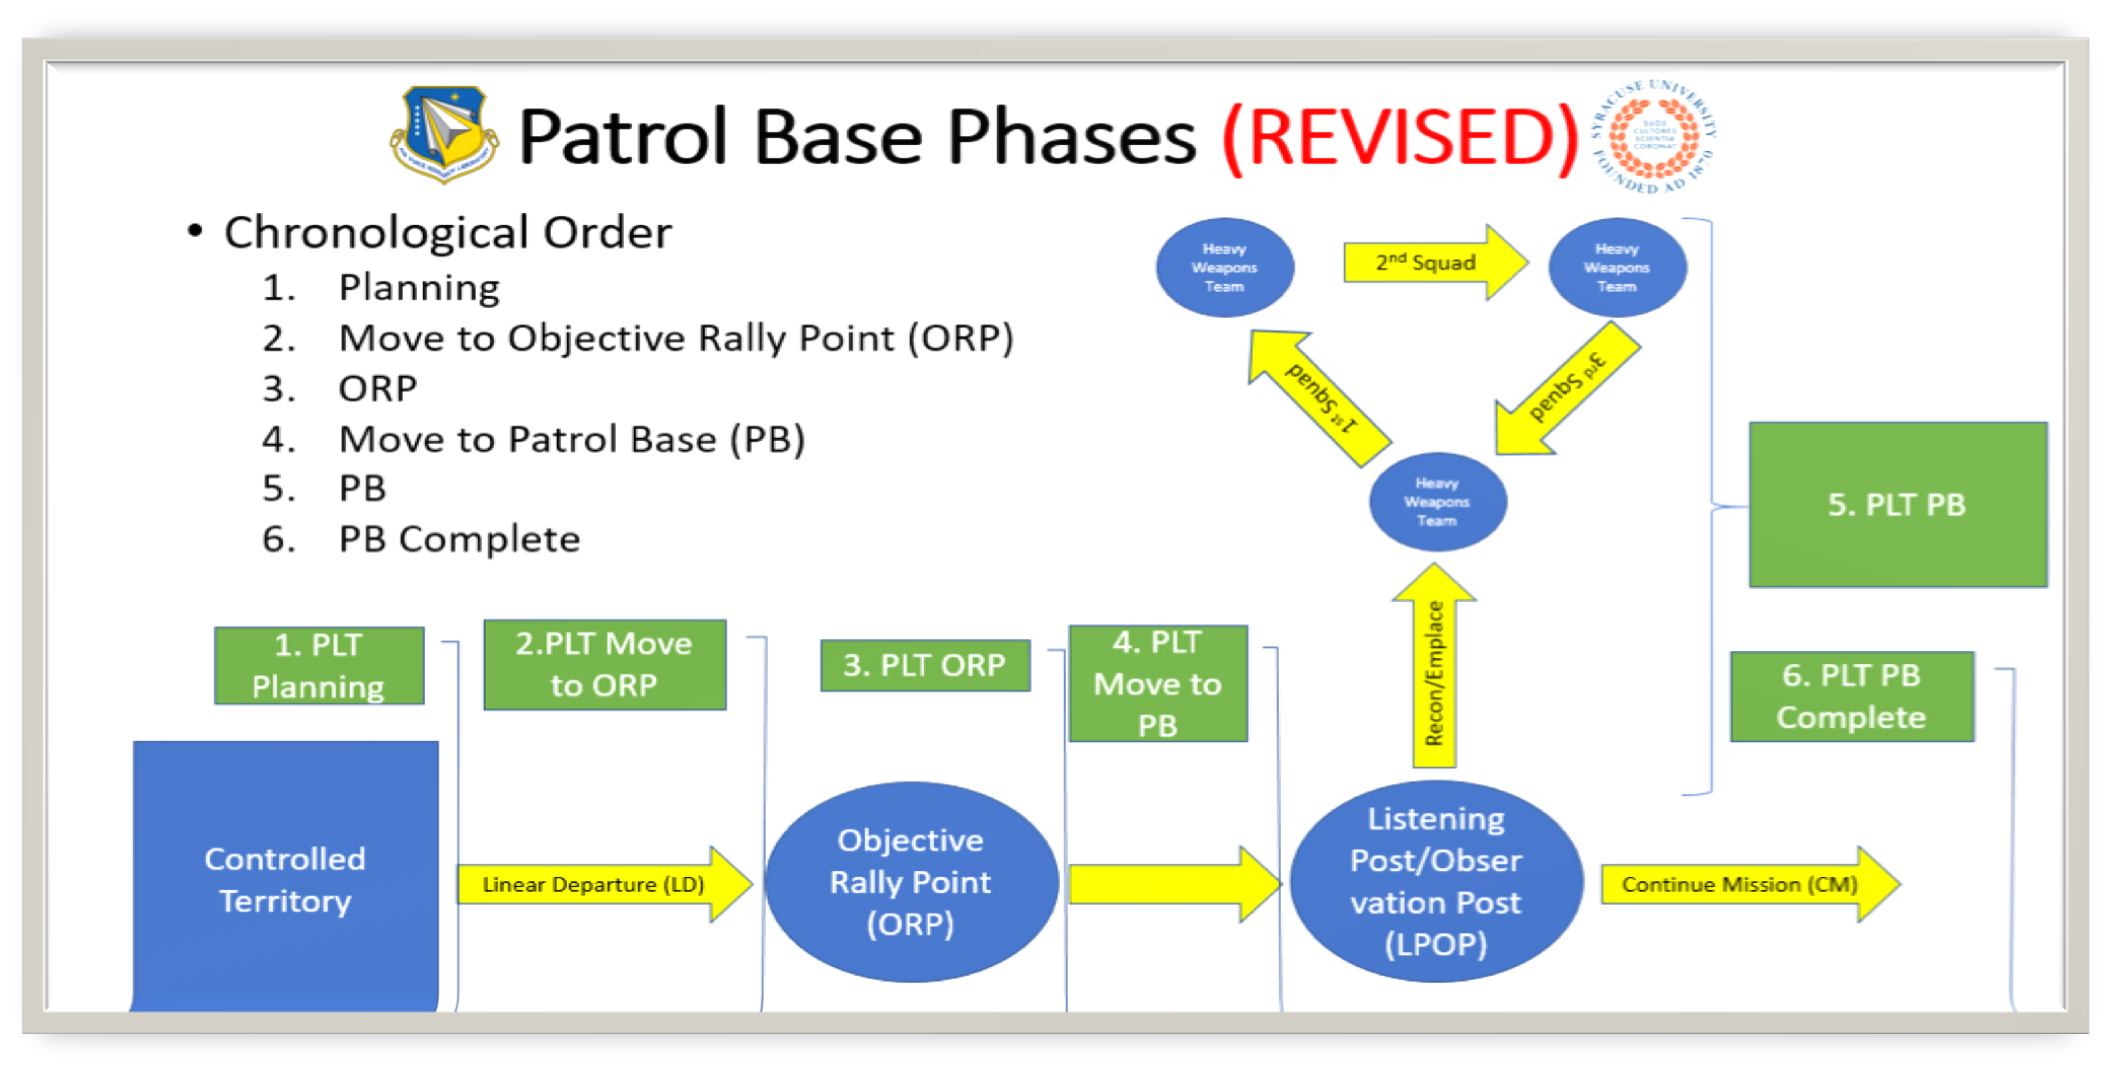
\includegraphics[width=\textwidth]{../figures/pbtoplevel}
\caption{\label{pbtoplevel2}A diagram of the most abstract level in the hierarchy of secure state machines.  Image generated by Jesse Nathaniel Hall.}
\end{figure}


\subsection{Transition Commands}
Transition commands are inputs to the state machine.  These inputs determine the next-state and next-output of the state machine.  To continue with the examples above, input for the transition from the n \textit{foreign civilians} state to the n + 1 \textit{foreign civilians}state could be ``access granted."  This same input could be used to change a foreign civilian's state from ``not granted" to ``granted."

In this master thesis, inputs are commands to transition from one state to another.  For example, in figure \ref{pbtoplevel2}, transition from the \textit{Move to Objective Rally Point (\gls{orp})} state to the \textit{\gls{orp}} state is indicated by the command ``conductORP."

\subsection{Next-state Function}
The next-state function (\textit{NS}) describes the next state of the state machine given the current state and input.   In \gls{hol} (and functional programming languages in general), the parameters follow the name of the function. \[ \text{\textit{NS CURRENT_STATE input }}\].  The function is defined with it's result.
\[ \text{\textit{NS CURRENT_STATE input = NEXT_STATE}}\]
For example, the next-state function to change from the n \textit{foreign civilians} state to the n + 1 \textit{foreign civilians} state using the "accessGranted" input would look like this: \[\text{\textit{NS N accessGranted = N + 1}}\]  Similarly, for the foreign civilian to change from the \textit{Not Granted} state to the \textit{Granted} state: \[\text{\textit{NS NOT_GRANTED accessGranted = GRANTED}}\].

In this master thesis, to transition from the \textit{MOVE_TO_ORP} state to the \textit{CONDUCT_ORP} state using the command "conductORP" looks like this:  \[\text{\textit{NS MOVE_TO_ORP conductORP = CONDUCT_ORP}}\]

\subsection{Next-output Function}
The next-output function (\textit{NSOut}) describes the next output of the state machine given the current state and input.  This is defined similarly to the next-state function.  \[\text{\textit{NOut CURRENT_STATE input = NextOutput}}\] 
For example, the next-output function to change from the n \textit{foreign civilians} state to the n + 1 \textit{foreign civilians} state using the "accessGranted" input would look like this: \[\text{\textit{NOut N accessGranted = BasePopulationIncreasedByOne}}\] Similarly, for the foreign civilian to change from the \textit{Not Granted} state to the \textit{Granted} state:: \[\text{\textit{NOut NOT_GRANTED accessGranted = NowOnBase}}\].

In this master thesis, the next output for the transition from the \textit{MOVE_TO_ORP} state to the \textit{CONDUCT_ORP} state using the command "conductORP" looks like this: 
\[\text{\textit{NS MOVE_TO_ORP conductORP = ConductORP}}\]

\subsection{Configuration}
A configuration describes the state machine using input and output streams \cite{certmanual}. A configuration has there components: (1) current state, (2) a list of inputs (input stream), and (3) a list of outputs (output stream). The information in the configuration is sufficient to instruct the state machine's behavior.

\subsection{TR Relations}
\Glspl{tr} define the behavior of the state machine based on its input, configuration, and the next configuration.  A \gls{tr} takes an input, an initial configuration, and a final configuration.  In terms of logic, a \gls{tr} is a propositional statement that is either true or false.  If the final configuration follows from the initial configuration and the input, then the \gls{tr} is true. Otherwise, it is false.  The trueness or falsity of the \gls{tr} follows from the next-state and next-output functions. The pattern looks like this:

\emph{
TR input\\
\hspace{0.5cm}CFG \\
\hspace{1.5cm}input::inputList\\
\hspace{1.5cm}CURRENT_STATE\\
\hspace{1.5cm}outList\\
\hspace{0.5cm}CFG\\
\hspace{1.5cm}inputList\\
\hspace{1.5cm}(NS input CURRENT_STATE)\\
\hspace{1.5cm}(NOut input CURRENT_STATE )::outList
}

\emph{CFG} is a type constructor\footnote{\see appendix \ref{sec:adtinml} for a description of types in \gls{hol}.} for a configuration.  What follows are the three components of the \emph{CFG} data type.  The first is the input stream, a list of inputs, denoted \emph{input::inputList}.\footnote{In functional programming languages, functions are applied to list elements one element at a time.  The notation headOfList::remainderOfList allows access to the first component of the list.}  The first component of this list is the same as the input to the TR.  The next component of the configuration is the current state, denoted \emph{CURRENT_STATE}.  The third component is the output list, denoted \emph{outList}.\footnote{Note that only the input (not the output) is needed for the \gls{tr} to evaluate to true or false. Therefore, the output is not denoted as headOfList::remainderOfList.}.  

The second \emph{CFG} is also composed of three components.  The first is the input list with the first element removed (because we used this element as input to the \gls{tr}).  The next component is the state which results from applying the \emph{input} and \emph{CURRENT_STATE} to the next-state function.  The third component is the output which results from applying the \emph{input} and \emph{CURRENT_STATE} to the next-state function.  This result is "consed" onto \emph{outList}.\footnote{"Consed" is functional programming language jargon for "appended to the front of the list."}

The input stream in the first configuration is a list (denoted as headOfList::remainderOfList).  Using an input stream, the next configuration can be defined using the remainder of the input stream (which could be the empty list) inputList as its input. 

The state in the first configuration is just the current state.  The next state in the final configuration is the result of the next-state function \textit{NS input CURRENT_STATE}.

The output in the first configuration is the outputList.  It's head should be the output that corresponds to the current state.  The output in the final configuration is the result of the next-output function cons'd onto the front of the outputList.

\glspl{tr} form the basis for the \glsentryshort{hol} representation of state machines, which is a precursor to the secure state machines implemented in this master thesis.  


      %%%%%%%%%%%%%%%%%%% Section Secure State Machines %%%%%%%%%
\section{Secure State Machines}\label{sec:ssm}
The secure state machine (\gls{ssm}) adds security to the state machine model.  It implements complete mediation using a monitor that verifies the authentication and authorization of any request (input) to transition from one state (or configuration) to another.   

\subsection{State Machine Versus Secure State Machine}
State machines define states, inputs, outputs, next-state functions, and next-output functions.  Through these means, the state machine defines it's behavior.  Secure state machines add the additional concept of complete mediation to the state machine model by including checks on authentication and authorization.  These checks are performed by a monitor.  A diagram showing the relationship between state machine and secure state machine with a monitor is shown in figure \ref{smVSssm}.  

\begin{figure}[!h!]
\centering
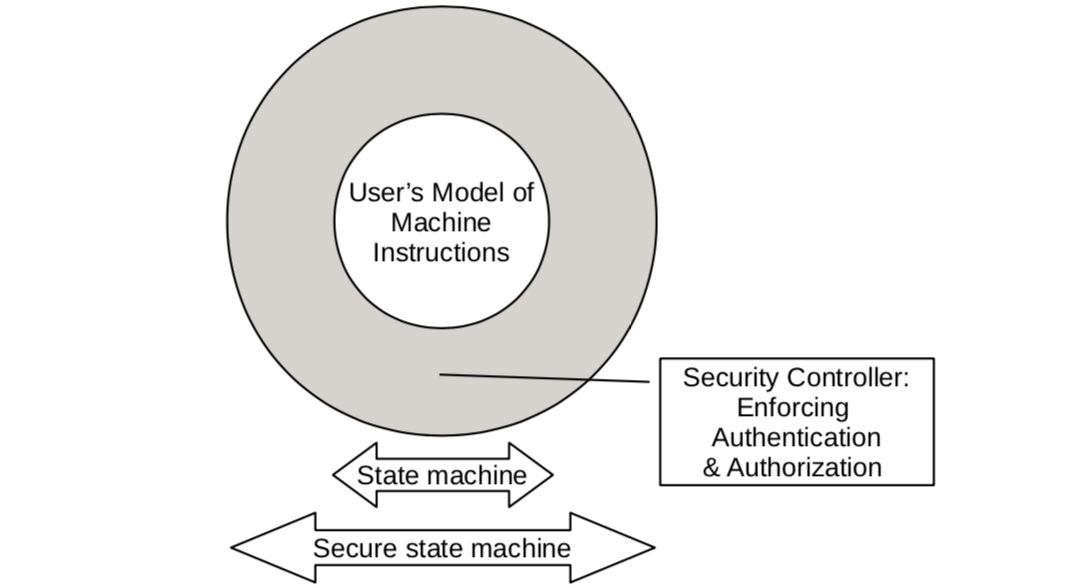
\includegraphics[width=0.8\textwidth]{../figures/smVSssm}
\caption{\label{smVSssm} State machine versus secure state machine with a monitor.  Image taken from Certified Security by Design Using Higher Order Logic \cite{certmanual}.}
\end{figure}

For this master thesis, the "Machine Instructions" represent the state machine model of the patrol base operations.


 
\subsection{Monitors}\label{monitors}
It is the duty of the monitor to control the behavior of the \gls{ssm} with regards to complete mediation.  The monitor is a essentially a guard that checks for the proper authentication and authorization for requests to access or change the state of the \glspl{ssm}.  In a real world analogy, the monitor is the sentry at the gate who checks IDs to verify a person's identify and checks with policy or procedures to determine if that person should be granted access.  

\subsection{Transition Types}
The monitor assigns a transition type to each command.  The transition types are: execute (\textit{exec}), trap, (\textit{trap}), and discard (\textit{discard})\footnote{The names are derived from their use in virtual machines.  Commands (inputs) in virtual machines are either executed, trapped, or discarded.  Each has a different behavior in the machine.}.  These correspond to executing a command, trapping a command, or discarding a command, respectively.  For example, \textit{exec accessGranted} indicates that the command to grant access for the foreign civilian to the base should be executed (or allowed).  \textit{trap accessGranted} means that the request to grant access is not authorized.  \textit{discard grantAccess} means that the command to grant access is not authenticated (i.e., the requestor's identify is not confirmed).

\subsection{Commands}
Commands in the \glsentryshort{ssm} are handled differently than in the state machine.  Principals issue commands (make requests).  The monitor inspects the command (request) for proper authentication and authorization and assigns a transition type to the command (request).  This combination of transition type and command (request) is then passed to the next-state and next-output functions.  These functions define how the \gls{ssm} responds to each transition type and command (request) pair.  

\subsection{Principals And Requests}
Principals are unique to the secure state machine.  The \gls{ssm} monitor checks authentication and authorization for each request.  This means the identify of "who" is making the request must be first verified and then authorized to control actions on the \gls{ssm}.  Therefore, a "who" must be defined.  The "who" in the access-control logic is the principal.  

Transitions in the \gls{ssm} are requested by a principal as \textit{Principal says changeStates}.  The next example shows how requests are made in a \gls{ssm} for the top level patrol base operations.

\begin{figure}[h!]
\centering
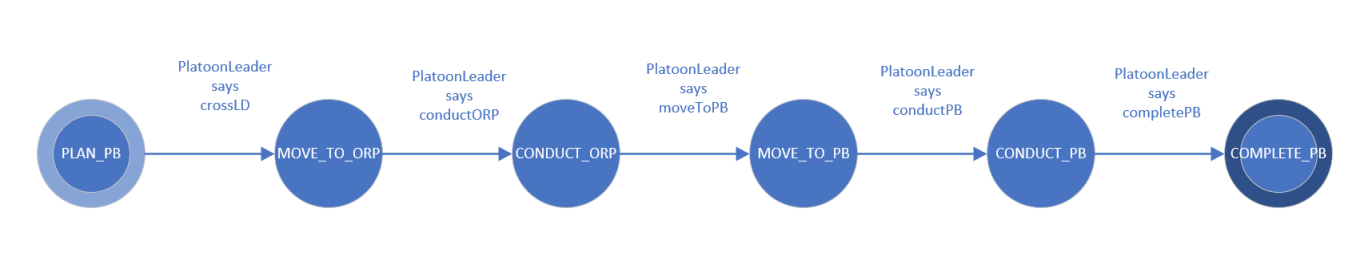
\includegraphics[width=\textwidth]{../figures/ssmPBDiagram}
\caption{\label{ssmPBDiagram2} Top level diagram.}
\end{figure}

Figure \ref{ssmPBDiagram2} shows the top level \gls{ssm}.  The transition from PLAN_PB to MOVE_TO_ORP in a state machine only requires the command \textit{crossLD}.  But, in the secure state machine, this transition looks like this:
 \[\textit{PlatoonLeader says crossLD}.\]

The monitor then checks the authentication and authorization of the principal and returns the command with a transition type.  For example, if the Platoon Leader is both authenticated and authorized on the command \textit{crossLD}, then the monitor returns the transition type and command pair 
\[exec \hspace{0.2cm} crossLD\]

This is passed to the next-state and next-output functions, which define the behavior for the command \textit{exec crossLD}.  Note that the next-state and next-output functions must also define the \gls{ssm} behavior for \textit{trap crossLD} and \textit{discard crossLD}.

\subsection{Authentication}
Authentication refers to verification of identity.\footnote{Authentication is a very broad topic and a thorough discussion is beyond the scope of this master thesis.}  Authentication is verified by the monitor for each request. 

In this master thesis, authentication is verified by visual confirmation of a principal's identity.  Either the monitor recognizes the principal making the request or not.\footnote{\glspl{ssm} also work with cryptographic functions. There already exists cryptographic versions of the \gls{ssm} described in this and the next section.}  The implementation of this in \gls{hol} authenticates principals on particular commands (or sets of commands).  Thus, the monitor authenticates the request \textit{SomePrincipal says someCommand} rather than just the \textit{SomePrincipal}. 


\subsection{Authorization}
Authorization controls access-rights by way of a security policy.  Authorization in the \gls{ssm} is defined by two functions.  One function describes access-control rules that are dependent on state and input.  The other function describes access-control rules that are dependent on only input only.  

Rules are of the form \textit{SomePrincipal controls someCommand}.  or \textit{if (state = SOME_STATE then SomePrincipal controls someCommand}.

With authentication and authorization rules defined, the \gls{ssm} monitor can use the \textit{Controls} rule described in section \ref{ssec:inferencerules} of chapter \ref{chp:csbdacl}.  Thus, the monitor reasons about a request and a policy as such:
\[\text{\textit{SomePrincipal says someCommand}}\]
\[\text{\textit{and}}\]
\[\text{\textit{SomePrincipal controls someCommand}}\]
\[\text{\textit{implies}}\]
\[\text{\textit{someCommand}}\]

More complicates statements that reduce to this are also allowed.

\subsection{Next-state And Next-output Functions}
The next-state and next-output functions define the behavior for the \gls{ssm}.  Whereas the behavior of the state machine is defined only for states and commands, the behavior in the \gls{ssm} includes the behavior for each transition type in combination with each command.  This means that for each command, the next-state and next-output functions define three separate behaviors: \textit{exec someCommand}, \textit{trap someCommand}, and \textit{discard someCommand}.  

\subsection{Configurations}
The configuration in the secure state machine adds three additional components, for a total of six: (1) an authentication function, (2) a state interpretation function (a state-dependent security policy), (3), a security context, (4) an input list (a command list), (5) a state, and (6) an output list.   The next-state and next-output functions are not part of the configuration because they define the permanent structure of the \gls{ssm}.

\subsection{TR Relations}
Transition relations in the secure state machine are similar to those for the state machine.  

\emph{
TR (trTpye input)\\
CFG \\
\hspace{1cm}authenticationTest\\
\hspace{1cm}stateInterpretation\\
\hspace{1cm}securityContext\\
\hspace{1cm}input::inputList\\
\hspace{1cm}CURRENT_STATE\\
\hspace{1cm}outList\\
CFG\\
\hspace{1cm}authenticationTest\\
\hspace{1cm}stateInterpretation\\
\hspace{1cm}securityContext\\
\hspace{1cm}inputList\\
\hspace{1cm}(NS (trType input) CURRENT_STATE)\\
\hspace{1cm}(NOut (trType input) CURRENT_STATE )::output
}

In addition to the three additional components (authenticationTest, stateInterpretation, and securityContext functions), the transition type (trType) is added to the front of the input. 

\subsection{Configuration Interpretation}
The TR relation is a proposition that returns true or false based on whether the second configuration follows from the first.  But, this is not wholly sufficient to prove complete mediation.  Complete mediation requires that the configuration be interpreted in the context of authentication and authorization.  The configuration interpretation function \emph{ConfigInterp} interprets the authentication and authorization of the request based on the current configuration.  

\emph{
ConfigInterp\\
\hspace{1cm}(M,Oi,Os)\\
\hspace{1cm}CFG\\
\hspace{2cm}AuthenticationTest inputOK\\
\hspace{2cm}StateInterpretation \\
\hspace{2cm}SecurityContext\\
\hspace{2cm}input::inputList\\
\hspace{2cm}CURRENT_STATE\\
\hspace{2cm}outList\\
\hspace{1cm}\HOLSymConst{\HOLTokenEquiv{}}\\
\hspace{1cm} (M,Oi,Os) satisfies (securityContext, input, and stateInterpretation)
}

Like \gls{tr}, this is higher order logic predicate that is either true or false.  It is a biconditional (if and only if).  If the first part of the bioconditional follows from the second and vis-a-vis, then the \emph{ConfigInterp} evaluates to true.  Otherwise, it evaluates to false.  It also requires use of the Kripke structure because it uses the \gls{acl} inference rules to evaluate.  

The first part of the bioconditional takes the current \emph{CFG}.  Note that in this \emph{CFG} the input is in the form of a request (not trType command).  

The second part of the biconditional is the "satisfies list."  This is a conjunction of the "satisfies" property applied to the securityContext, input, and StateInterpretation function. The \emph{SecurityContext} and \emph{StateInterpreation} functions are user defined and specific for each state machine.


      %%%%%%%%%%%%%%%%%%% Section SSMs in HOL %%%%%%%%%%%%%
\section{Secure State Machines in HOL}\label{sec:sminHOL}
This following sections describe the \gls{hol} implementation of the \gls{ssm}.  It focuses on the parametrizable \gls{ssm} that forms the basis for the patrol base operations \glspl{ssm} described in the next chapter.  The parametrizable \gls{ssm} is denoted as "ssm".

\subsection{Parameterizable Secure State Machine}
ssm is implemented as a parametrizable secure state machine. Parametrization allows for re-use of common definitions and theorems in the \glsentryshort{ssm} model.  The parametrizable components are
\begin{itemize}
\item Next-state function
\item Next-output function
\item Input \& Input stream
\item Output \& Output stream
\item States
\item Principals
\item Security context
\item State interpretation-based security context
\item Authentication test function
\end{itemize}

%To use the ssm, the rule ISPECL \glsentryshort{hol} is used to specialize the parametrizable theorems for a specific secure state machine. 

\subsection{Input Stream}
The input to the secure state machines is in the form of a list of inputs (an input stream).  Elements in the list are of the form \textit{P says prop (SOME cmd)}\footnote{See next section.}.  It is necessary to extract particular components from the list and list elements.  Several functions are defined to do this.  These are essentially helper functions.

\paragraph*{extractCommand}
extractCommand takes one input of the form \textit{P says prop (SOME cmd)} and extracts the \textit{cmd} part.

\HOLThmTag{ssm}{extractCommand_def}\HOLssmTheoremsextractCommandXXdef


\paragraph*{commandList}
commandList takes an input list consisting of list elements of the form \textit{P says prop (SOME cmd)}.  It returns a list of all the \textit{cmd} elements.
\begin{tabbing}
\parskip=8pt
\HOLTokenTurnstile{} \HOLSymConst{\HOLTokenForall{}}\HOLBoundVar{x}. \\
\hspace{0.3cm} \HOLConst{commandList} \HOLBoundVar{x} \HOLSymConst{=} \HOLConst{MAP} \HOLConst{extractCommand} \HOLBoundVar{x}
\parskip=18pt
\end{tabbing}

\paragraph*{extractPropCommand}
extractPropCommand takes one input of the form \textit{P says prop (SOME cmd)} and extracts the \textit{prop (SOME cmd)} part.

\HOLThmTag{ssm}{extractPropCommand_def}\HOLssmTheoremsextractPropCommandXXdef


\paragraph*{propCommand}
propCommand takes an input list consisting of list elements of the form \textit{P says prop (SOME cmd)}.  It returns a list of all the \textit{prop (SOME cmd)} elements.
\begin{tabbing}
\parskip=8pt
\HOLTokenTurnstile{} \HOLSymConst{\HOLTokenForall{}}\HOLBoundVar{x}. \\
\hspace{0.3cm} \HOLConst{propCommandList} \HOLBoundVar{x} \HOLSymConst{=} \HOLConst{MAP} \HOLConst{extractPropCommand} \HOLBoundVar{x}
\parskip=18pt
\end{tabbing}


\paragraph*{extractInput}
extractInput takes one input of the form \textit{P says prop x} and extracts the \textit{x} part. Note that \textit{x} can have two forms: \textit{NONE} or \textit{SOME cmd}.

\HOLThmTag{ssm}{extractInput_def}\HOLssmTheoremsextractInputXXdef


\paragraph*{inputList}
inputList takes an input list consisting of list elements of the form \textit{P says prop x}.  It returns a list of all the \textit{x} elements.
\begin{tabbing}
\parskip=8pt
\HOLTokenTurnstile{} \HOLSymConst{\HOLTokenForall{}}\HOLBoundVar{xs}. \\
\hspace{0.3cm} \HOLConst{inputList} \HOLBoundVar{xs} \HOLSymConst{=} \HOLConst{MAP} \HOLConst{extractInput} \HOLBoundVar{xs}
\parskip=18pt
\end{tabbing}


\subsection{Commands}
\paragraph*{Option Type}\label{option}
The option type allows for the return of \textit{SOME command} or \textit{NONE}.  For example, \textit{P says prop (SOME cmd)} or \textit{P says prop NONE}.  Option types are common in functional programming languages because a function must return something.  The \textit{NONE} option allows for that something to be nothing.


The definition for the option datatype is

\HOLFreeVar{option} = \HOLConst{NONE} \HOLTokenBar{} \HOLConst{SOME} 'a

In the datatype definition above, 'a is replaced with some other datatype.  

\paragraph*{A Closer Look at Commands}
To see what this looks like in \glsentryshort{hol}, it is necessary to define some other datatypes. The OMNILevel folder in OMNITypesScript.sml contains definitions that are used in all patrol base operations \glsentryshortpl{ssm}. One definition is the \HOLFreeVar{command} datatype definition.

\begin{tabbing}
\HOLFreeVar{command} = \HOLConst{ESCc} \HOLTyOp{escCommand} \HOLTokenBar{} \HOLConst{SLc} 'slCommand
\end{tabbing}

The \HOLFreeVar{command} datatype consists of two additional datatypes: \HOLConst{ESCc} \HOLTyOp{escCommand} and \HOLConst{SLc} 'slCommand.  Note that the first part of each of these are the datatype constructors\footnote{see the background section \ref{sec:adtinml}}: \HOLConst{ESCc} and \HOLConst{SLc}.  The second part is the name of the datatype variable\footnote{Both of these are datatype variables because they define other datatypes.} or datatype.  

The first datatype refers to the escape commands.  They are defined as \HOLTyOp{escCommand} in the same file as \HOLFreeVar{command}.

 \begin{tabbing}
 \HOLFreeVar{escCommand} = \= \HOLConst{returnToBase} \\
 						\>\HOLTokenBar{} \HOLConst{changeMission} \\
						\>\HOLTokenBar{} \HOLConst{resupply}\\
           					\>\HOLTokenBar{} \HOLConst{reactToContact}
\end{tabbing}

This datatype definition defines three commands (or datatype values) which represent escape conditions in the patrol base operations.  

The second dataytpe variable 'slCommand refers to the state-level commands.  These are defined further in each \glsentryshort{ssm}.  

Notice that there is a tick mark (apostrophe) before 'slCommand and not before \HOLTyOp{escCommand}.  In general, the tick mark in \glsentryshort{hol} represents an undefined dataytpe.  In this case, 'slCommand is not yet defined (because it is defined elsewhere), whereas the definition for \HOLTyOp{escCommand} is defined in the same file and above the definition for \HOLFreeVar{command}.   

An example of a definition for 'slCommand can be found in the top level \glsentryshort{ssm}.  It is defined in the folder topLevel and in the file PBIntegratedTypeScript.sml file.

\HOLFreeVar{slCommand} = \HOLConst{PL} \HOLTyOp{plCommand} \HOLTokenBar{} \HOLConst{OMNI} \HOLTyOp{omniCommand}

This is defined similarly to \HOLFreeVar{command}.  There are two datatypes that make-up the datatype \HOLFreeVar{slCommand}.  None of these have tick marks, which means both of these are defined.  In particular, they are both defined in the same file as \HOLFreeVar{slCommand}.

\HOLFreeVar{plCommand} refers to the Platoon Leader commands.  These are commands that the Platoon Leader is authorized to make.  These are not data type variables, they are data types, because they are not further defined.

\begin{tabbing}
\HOLFreeVar{plCommand} = \= \HOLConst{crossLD} \\
					     \>\HOLTokenBar{} \HOLConst{conductORP} \\
					     \>\HOLTokenBar{} \HOLConst{moveToPB} \\
					     \>\HOLTokenBar{} \HOLConst{conductPB}\\
         				     \> \HOLTokenBar{} \HOLConst{completePB} \\
				             \> \HOLTokenBar{} \HOLConst{incomplete}
\end{tabbing}


\HOLFreeVar{omniCommand} refers to commands that the OMNI level principal\footnote{See section \ref{ssec:omnilevel} for a discussion of the OMNI level principal.} is authorized to make. 

\begin{tabbing}
\HOLFreeVar{omniCommand} = \= \HOLConst{ssmPlanPBComplete} \\
						 \> \HOLTokenBar{} \HOLConst{ssmMoveToORPComplete}\\
 				       	 	 \> \HOLTokenBar{} \HOLConst{ssmConductORPComplete} \\
						 \> \HOLTokenBar{} \HOLConst{ssmMoveToPBComplete}\\
            					 \> \HOLTokenBar{} \HOLConst{ssmConductPBComplete}\\
					 	 \> \HOLTokenBar{} \HOLConst{invalidOmniCommand}
\end{tabbing}          
          
          
\paragraph*{Option Type with Commands}
With these definitions, it is possible to see how the options types are used with commands (datatypes).  What follows is a list of examples using the option types and commands (datatypes) described above.  The type signatures are also included because it will help the reader recognize them in the \gls{hol} code.
\begin{description}
\item[ ] SOME (SLc (ESCc returnToBase)) \\
The type for this is (escCommand command)Option.
\item[ ] SOME (SLc (PL moveToORP))  \\
The type for this is ((plCommand slCommand) command)Option.  
\item[ ] SOME (SLc (OMNI ssmMoveToORPComplete))\\
The type for this is ((omniCommand slCommand) command)Option.  
\end{description}

Note that the constructors are necessary for each command. Also, note that in the \gls{hol} code for the patrol base operations, the reader will typically see \textit{(slCommand command)Option} rather than \textit{((plCommand slCommand) command)Option}, for example.  This is because most of the authentication and authorization definitions require a type \HOLFreeVar{slCommand}, which includes both \HOLFreeVar{plCommand}  and \HOLFreeVar{omniCommand}.




\subsubsection{Transition Types}
Transition datatypes indicate how a command is handled by the monitor.  The three transition datatypes are described below. 

\HOLFreeVar{trType} = \HOLConst{discard} 'cmdlist \HOLTokenBar{} \HOLConst{trap} 'cmdlist \HOLTokenBar{} \HOLConst{exec} 'cmdlist

The 'cmdlist refers to a list of commands of the form discussed in the section above.  For example, to execute the transition from the PLAN_PB state to the MOVE_TO_ORP state, the monitor must return the transition type and command pair with the later of the pair in the form of a list 
\[\text{\textit{exec [SOME (SLc (PL crossLD))]}} \]

where \textit{SOME (SLc (PL crossLD))} is the single item in the cmdlist.  The transition type with the command list is then passed to the next-state and next-output functions.  The transition from the WARNO to the REPORT1 state in ssmPlanPB requires four commands.
\[\text{\textit{exec [SOME (SLc (PL crossLD)); SOME (SLc (PL crossLD));}} \]
\[\text{\textit{SOME (SLc (PL crossLD)); SOME (SLc (PL crossLD))]}} \]

List elements are separated with a semicolon.

\subsection{Authentication}
Authentication is context dependent. But, a parametrizable authentication function is defined in the parametrizable \gls{ssm}.

\begin{tabbing}
\parskip=8pt

\HOLTokenTurnstile{} \=\HOLSymConst{\HOLTokenForall{}}\HOLBoundVar{elementTest} \HOLBoundVar{x}. \\
    \> \HOLConst{authenticationTest} \HOLBoundVar{elementTest} \HOLBoundVar{x}  \HOLSymConst{\HOLTokenEquiv{}} \\
    \> \HOLConst{FOLDR} (\HOLTokenLambda{}\HOLBoundVar{p} \HOLBoundVar{q}. \HOLBoundVar{p} \HOLSymConst{\HOLTokenConj{}} \HOLBoundVar{q}) \HOLConst{T} (\HOLConst{MAP} \HOLBoundVar{elementTest} \HOLBoundVar{x})
\parskip=18pt
\end{tabbing}

This function takes an \texttt{elementTest} function and an input list as parameters.  The \texttt{elementTest} function is named \texttt{inputOK} in the patrol base operations \glspl{ssm} and it is defined separately for each \gls{ssm}.  \texttt{elementTest} takes a single input of the form \textit{SomePrincipal says someCommand}.  It returns TT (the \gls{acl} representation of True) if the input is authenticated and FF otherwise.  

The authenticationTest function FOLDRs the elementTest function over the input list x with the conjunction function and True as the accumulator\footnote{This means that the elementTest function is applied to each element in the input list x, resulting in a TT or FF value for each element in the input list x.   Then, in essence, the value of the conjunction of all these values is returned.}  Thus, if all the input elements in the input list x pass the elementTest, the authenticationTest function returns true, otherwise it returns false.  
     
\subsection{Authorization}
Authorization is the security context and it is \gls{ssm}-dependent. This means that each \gls{ssm} defines its own security context.  The parametrizable \gls{ssm} allows for two ways to define the security context and pass them as parameters.  The first is the state interpretation function. This function takes a state and an input list as parameters.  It defines the security context based on state.  All state-dependent behavior may also be defined in this function.

The second function is the security context function.  It takes only the input list as a parameter.  It's definition applies to all states.

\subsection{Next-state And Next-output Functions}
The next-state and next-output functions are parameters to the parametrizable \gls{ssm}.  They are defined separately in each \gls{ssm}.  In the parametrizable \gls{ssm} they are denoted by NS and Out, respectively.

\subsection{Configurations}
Configurations in the \glspl{ssm} have six components.  Each \gls{ssm} must define all six components to use the parametrizable ssm.  These components are:
\begin{enumerate}
\item authentication test function.  \\
The type signature is 

\hspace{0.5cm}  (('command \HOLTyOp{option}, 'principal, 'd, 'e) \HOLTyOp{Form} -> \HOLTyOp{bool})

\item state interpretation function.  \\
The type signature is
\begin{tabbing}
\hspace{0.5cm}('state -> \=('command \HOLTyOp{option}, 'principal, 'd, 'e) \HOLTyOp{Form} \HOLTyOp{list} -> \\
				      \>('command \HOLTyOp{option}, 'principal, 'd, 'e) \HOLTyOp{Form} \HOLTyOp{list}) 
\end{tabbing}
\item security context function.  \\
The type signature is 

 \hspace{0.5cm}   (('command \HOLTyOp{option}, 'principal, 'd, 'e) \HOLTyOp{Form} \HOLTyOp{list} -> \\
\hspace{0.5cm}    ('command \HOLTyOp{option}, 'principal, 'd, 'e) \HOLTyOp{Form} \HOLTyOp{list}) 

\item input list stream.  \\
The type signature is

 \hspace{0.5cm}  (('command \HOLTyOp{option}, 'principal, 'd, 'e) \HOLTyOp{Form} \HOLTyOp{list} \HOLTyOp{list}) \

\item state.  \\
The type signature is

\hspace{0.5cm}   'state

\item output stream.  \\
The type signature is 

\hspace{0.5cm} ('output \HOLTyOp{list})
\end{enumerate}

Note that the authentication test function is defined in the parametrizable ssm as authenticationTest.  This function takes one input (named elementTest in this ssm and inputOK in the \glsentryshortpl{ssm}).

These components comprise the six components of the configuration datatype (with CFG as the datatype constructor)

\begin{tabbing}
\parskip=8pt
\HOLFreeVar{configuration} = \\
\hspace{0.3cm}    \HOLConst{CFG} \\
\hspace{0.5cm}  (('command \HOLTyOp{option}, 'principal, 'd, 'e) \HOLTyOp{Form} -> \HOLTyOp{bool})\\
\hspace{0.5cm}    ('state -> ('command \HOLTyOp{option}, 'principal, 'd, 'e) \HOLTyOp{Form} \HOLTyOp{list} -> \\
\hspace{0.5cm}    ('command \HOLTyOp{option}, 'principal, 'd, 'e) \HOLTyOp{Form} \HOLTyOp{list}) \\
 \hspace{0.5cm}   (('command \HOLTyOp{option}, 'principal, 'd, 'e) \HOLTyOp{Form} \HOLTyOp{list} -> \\
\hspace{0.5cm}    ('command \HOLTyOp{option}, 'principal, 'd, 'e) \HOLTyOp{Form} \HOLTyOp{list}) \\
 \hspace{0.5cm}  (('command \HOLTyOp{option}, 'principal, 'd, 'e) \HOLTyOp{Form} \HOLTyOp{list} \HOLTyOp{list}) \\
\hspace{0.5cm}   'state \\
\hspace{0.5cm} ('output \HOLTyOp{list})
\parskip=18pt
\end{tabbing}

\subsection{Configuration Interpretation}
The monitor must interpret the configuration.  The CFGInterpret function take as input a Kripke structure and a configuration.  It returns a conjunction of three things: a satList of the security context, a satList of the input stream, and a satList of the stateInterpretation function.  

satList is a list of elements that satisfy the property of soundness as discussed in chapter \ref{chp:csbdacl} section \ref{sssec:soundness}\footnote{Note that in the \glsentryshort{acl} implementation of the "satisfies" and "soundness" properties, "satisfies" serves as "soundness" when it is generalized for all Kripke structures.}.  satList is defined in satListTheory.  

\begin{tabbing}
\parskip=8pt
\HOLTokenTurnstile{} \hspace{0.3cm}\HOLSymConst{\HOLTokenForall{}}\HOLBoundVar{M} \HOLBoundVar{Oi} \HOLBoundVar{Os} \HOLBoundVar{formList}.\\
\hspace{0.5cm}(\HOLBoundVar{M}\HOLSymConst{,}\HOLBoundVar{Oi}\HOLSymConst{,}\HOLBoundVar{Os}) \HOLConst{satList} \HOLBoundVar{formList} \HOLSymConst{\HOLTokenEquiv{}} \\
\hspace{0.5cm} \HOLConst{FOLDR} (\HOLTokenLambda{}\HOLBoundVar{x} \HOLBoundVar{y}. \HOLBoundVar{x} \HOLSymConst{\HOLTokenConj{}} \HOLBoundVar{y}) \HOLConst{T} (\HOLConst{MAP} (\HOLTokenLambda{}\HOLBoundVar{f}. (\HOLBoundVar{M}\HOLSymConst{,}\HOLBoundVar{Oi}\HOLSymConst{,}\HOLBoundVar{Os}) \HOLConst{sat} \HOLBoundVar{f}) \HOLBoundVar{formList})
\parskip=18pt
\end{tabbing}

satList MAPs the \textit{sat} operator onto each element in the formList. It then FOLDRs the formList elements with the conjunction function and accumulator True.  This means that satList applied to formList returns true if each element in the list satisfies the \textit{sat} property.

Other properties of satList can be found in appendix \ref{ppacl}.

With satList defined, the meaning of CFGInterpret should follow.  

\begin{tabbing}
\parskip=8pt
\HOLTokenTurnstile{} \HOLConst{CFGInterpret}\\
\hspace{0.5cm}(\HOLFreeVar{M}\HOLSymConst{,}\HOLFreeVar{Oi}\HOLSymConst{,}\HOLFreeVar{Os})
     (\HOLConst{CFG} \HOLFreeVar{elementTest} \HOLFreeVar{stateInterp} \HOLFreeVar{context} (\HOLFreeVar{x}\HOLSymConst{::}\HOLFreeVar{ins}) \HOLFreeVar{state}
     \HOLFreeVar{outStream}) \HOLSymConst{\HOLTokenEquiv{}} \\
\hspace{0.5cm}(\HOLFreeVar{M}\HOLSymConst{,}\HOLFreeVar{Oi}\HOLSymConst{,}\HOLFreeVar{Os}) \HOLConst{satList} \HOLFreeVar{context} \HOLFreeVar{x} \HOLSymConst{\HOLTokenConj{}} (\HOLFreeVar{M}\HOLSymConst{,}\HOLFreeVar{Oi}\HOLSymConst{,}\HOLFreeVar{Os}) \HOLConst{satList} \HOLFreeVar{x} \HOLSymConst{\HOLTokenConj{}}\\
\hspace{0.5cm}(\HOLFreeVar{M}\HOLSymConst{,}\HOLFreeVar{Oi}\HOLSymConst{,}\HOLFreeVar{Os}) \HOLConst{satList} \HOLFreeVar{stateInterp} \HOLFreeVar{state} \HOLFreeVar{x}
\parskip=18pt
\end{tabbing}


\subsection{TR Rules}\label{ssec:trrules}
The transition rules in \glsentryshort{hol} are defined in figure \ref{trrules}.

\begin{figure}[h!]
\centering
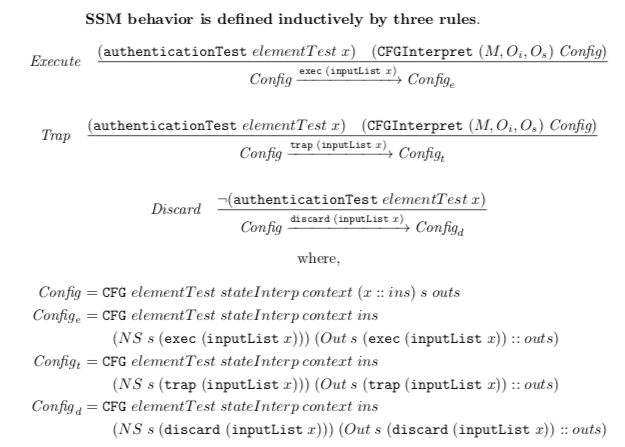
\includegraphics[width=\textwidth]{../figures/trrules}
\caption{\label{trrules} Transition rules in \glsentryshort{hol}.   Image taken from Certified Security by Design Using Higher Order Logic \cite{certmanual}}
\end{figure}

There are three rules, one for each transition type.  Above each line are the hypotheses and below are the conclusions.  The symbol $\text{\textit{Config}}  \xrightarrow[\text{}]{\text{exec (inputList x)}} \textit{Config}_e$ represents the TR relation for the input \textit{exec inputList x}.  Similarly, the symbols $\text{\textit{Config}}  \xrightarrow[\text{}]{\text{trap (inputList x)}} \textit{Config}_t$ and $\text{\textit{Config}}  \xrightarrow[\text{}]{\text{discard (inputList x)}} \textit{Config}_d$ represent the TR relations for \textit{trap inputList x} and \textit{discard inputList x}, respectively. 


The \textit{Execute} rule takes the authenticationTest function (with two parameters) and the CFGInterpret function (with two parameters).  If these are true, then \textit{Execute} concludes the TR relation $\text{\textit{Config}}  \xrightarrow[\text{}]{\text{exec (inputList x)}} \textit{Config}_e$.  \textit{Trap} is similar to \textit{Execute}.

The \textit{Discard} rule takes only the authenticationTest function (with two parameters).  If this is false, then the hypothesis is true.  Thus, the  $\text{\textit{Config}}  \xrightarrow[\text{}]{\text{discard (inputList x)}} \textit{Config}_d$ follows.

The definitions for the \textit{Config}s are defined below the rules. 

These definitions are defined in \glsentryshort{hol} as rule0, rule1, and rule2 (TR_discard_cmd_rule).  Notice that these are biconditionals.  The hypotheses and conclusions are reversed in the definitions below.  

\paragraph*{rule0}
\HOLThmTag{ssm}{TRrule0}\HOLssmTheoremsTRruleZero



\paragraph*{rule1}
\HOLThmTag{ssm}{TRrule1}\HOLssmTheoremsTRruleOne

\paragraph*{rule2}


\HOLThmTag{ssm}{rule2...(same as) TR_discard_cmd_rule}\HOLssmTheoremsTRXXdiscardXXcmdXXrule


\paragraph*{Complete mediation and TR Relations}
If remains to prove that complete mediation justifies execution, trapping, or discarding of commands. 

\paragraph*{TR_exec_cmd_rule}
The following function demonstrates the property of complete mediation as a condition for execution a command.


\HOLThmTag{ssm}{TR_exec_cmd_rule}\HOLssmTheoremsTRXXexecXXcmdXXrule

This is similar to rule0.  It adds the following as a premise for concluding rule0.

\HOLTokenTurnstile{} 
\HOLSymConst{\HOLTokenForall{}}\HOLBoundVar{elementTest} \HOLBoundVar{context} \HOLBoundVar{stateInterp} \HOLBoundVar{x} \HOLBoundVar{ins} \HOLBoundVar{s} \HOLBoundVar{outs}.\\
\hspace{0.5cm}(\HOLSymConst{\HOLTokenForall{}}\HOLBoundVar{M} \HOLBoundVar{Oi} \HOLBoundVar{Os}.\\
\hspace{0.9cm}\HOLConst{CFGInterpret} (\HOLBoundVar{M}\HOLSymConst{,}\HOLBoundVar{Oi}\HOLSymConst{,}\HOLBoundVar{Os})\\
\hspace{1.1cm}(\HOLConst{CFG} 
\HOLBoundVar{elementTest} 
\HOLBoundVar{stateInterp} 
\HOLBoundVar{context} 
(\HOLBoundVar{x}\HOLSymConst{::}\HOLBoundVar{ins}) 
\HOLBoundVar{s}
\HOLBoundVar{outs}) \\
\HOLSymConst{\HOLTokenImp{}}(\HOLBoundVar{M}\HOLSymConst{,}\HOLBoundVar{Oi}\HOLSymConst{,}\HOLBoundVar{Os}) \HOLConst{satList} \HOLConst{propCommandList} \HOLBoundVar{x}) \\

This part requires that the propCommandList applied to the inputList satisfies the Kripke structure.

\paragraph*{TR_trap_cmd_rule}
TR_trap_cmd_rule is similar to TR_exec_cmd_rule. 

\HOLThmTag{ssm}{TR_trap_cmd_rule}\HOLssmTheoremsTRXXtrapXXcmdXXrule

The difference is that instead of requiring propCommandList to satisfy the Kripke structure, it must satisfy NONE.  

\HOLTokenTurnstile{} 
\HOLSymConst{\HOLTokenForall{}}\HOLBoundVar{elementTest} \HOLBoundVar{context} \HOLBoundVar{stateInterp} \HOLBoundVar{x} \HOLBoundVar{ins} \HOLBoundVar{s} \HOLBoundVar{outs}.\\
\hspace{0.5cm} (\HOLSymConst{\HOLTokenForall{}}\HOLBoundVar{M} \HOLBoundVar{Oi} \HOLBoundVar{Os}.\\
\hspace{0.9cm}\HOLConst{CFGInterpret} (\HOLBoundVar{M}\HOLSymConst{,}\HOLBoundVar{Oi}\HOLSymConst{,}\HOLBoundVar{Os})\\
\hspace{1.1cm}(\HOLConst{CFG} 
\HOLBoundVar{elementTest} 
\HOLBoundVar{stateInterp} 
\HOLBoundVar{context} 
(\HOLBoundVar{x}\HOLSymConst{::}\HOLBoundVar{ins}) 
\HOLBoundVar{s}
\HOLBoundVar{outs}) \\
\HOLSymConst{\HOLTokenImp{}} (\HOLBoundVar{M}\HOLSymConst{,}\HOLBoundVar{Oi}\HOLSymConst{,}\HOLBoundVar{Os}) \HOLConst{sat} \HOLConst{prop} \HOLConst{NONE}) 



\paragraph*{TR_discard_cmd_rule}
This is the same as rule2 because the \textit{discard} transition type does not require configuration interpretation.


The next chapter demonstrates the parametrizable ssm applied to specific patrol base operations \glsentryshortpl{ssm}.
\end{document}